

Como dijimos antes, la complejidad del algoritmo es siempre $\Theta(n m)$, sin distinción entre casos, por lo que el análisis de performance es simple.

\begin{figure}[H]
 \centering
	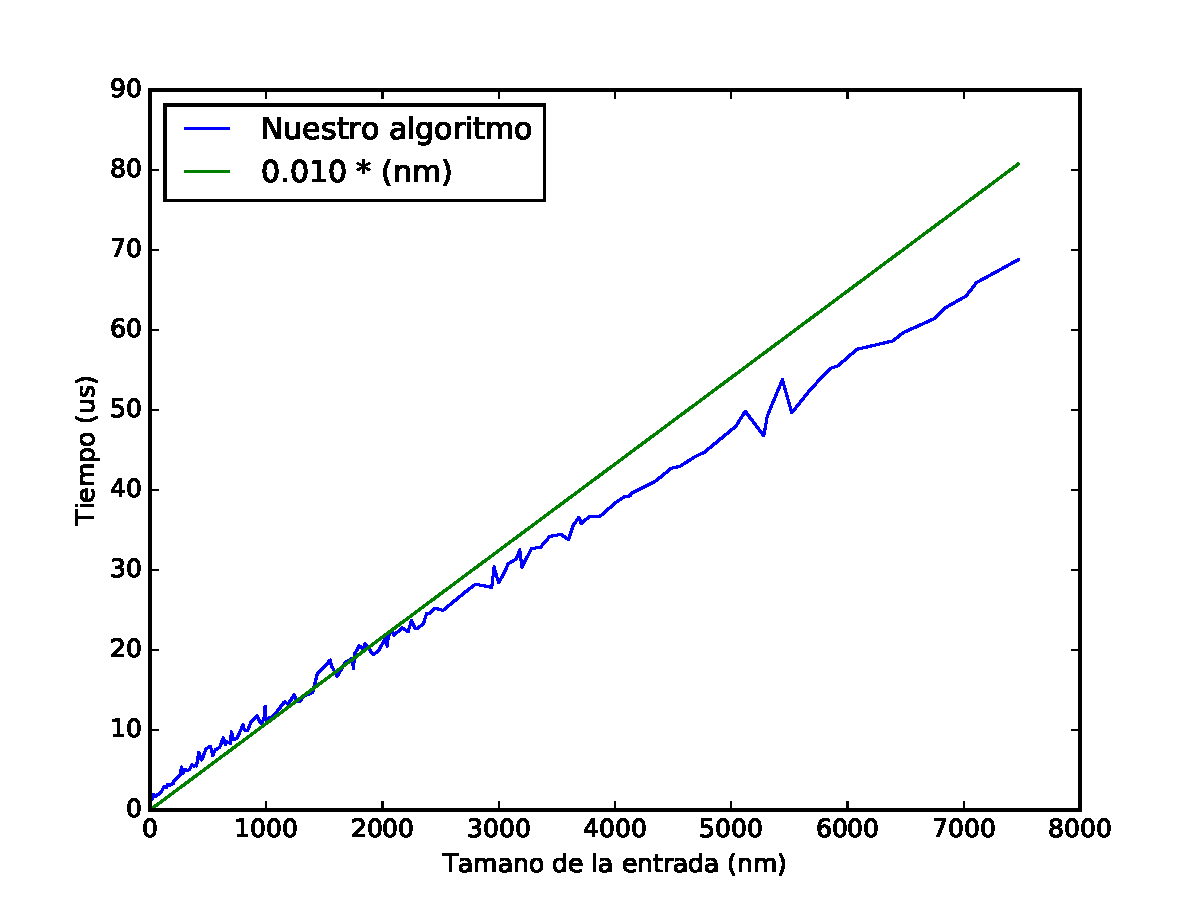
\includegraphics[width=0.9\textwidth]{img/exp/problema3-promedio.pdf}
	\caption{\footnotesize Tiempo que toma el algoritmo en $\mu$s para una entrada de tamaño $mn$.}
	\label{fig:problema3-promedio}
\end{figure}

En esta imagen se ve que se comporta como debe. Sin embargo, al igual que en los problemas anteriores, para confirmarlo totalmente, realizamos el gráfico de $\frac{T(nm)}{nm}$, dado que si esta función tiene a una constante cuando $nm \to \infty$, habremos confirmado experimentalmente que la complejidad del algoritmo es de $\Theta(n m)$.

\begin{figure}[H]
 \centering
	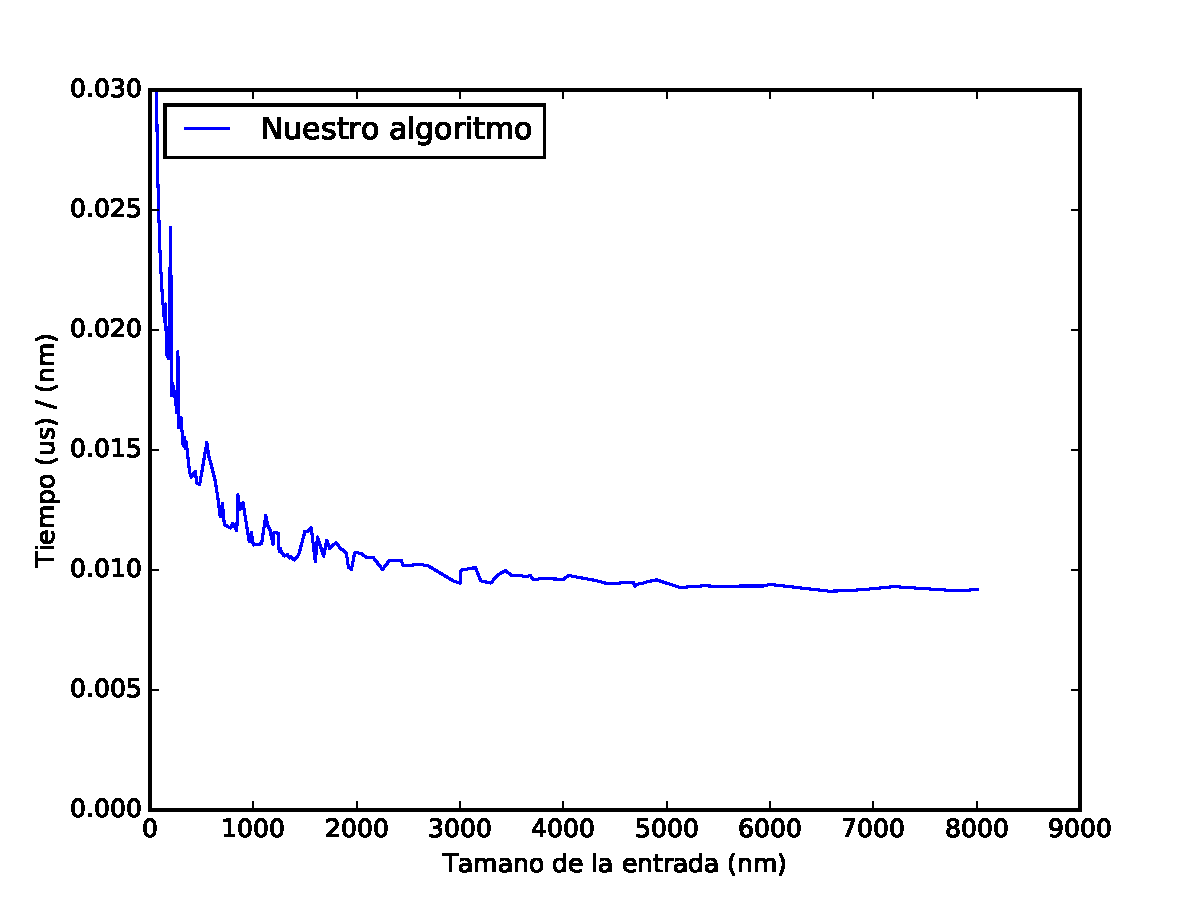
\includegraphics[width=0.9\textwidth]{img/exp/problema3-promedio2.pdf}
	\caption{\footnotesize Tiempo que toma el algoritmo en $\mu$s dividido $mn$ para una entrada de tamaño $mn$.}
	\label{fig:problema3-promedio2}
\end{figure}


\subsubsection{M\'etodo de experimentación}

Dados $n$ y $m$, generamos una matriz de $n \times m$, donde cada celda tiene un peso al azar. Para cada par $n$, $m$ generamos varias matrices (cada una con pesos distintos en cada celda), y tomamos la mediana de esas mediciones. 

De todas maneras, la varianza del tiempo para cada matriz de la misma dimensión era casi nula, dado que obviamente el valor de las celdas no afecta el tiempo. Sin embargo, nos parece importante aclarar que esto sucede, y que además fue verificado experimentalmente como dijimos.


